\chapter{Estado de la Cuestión}
\label{cap:estadoDeLaCuestion}

%%En el estado de la cuestión es donde aparecen gran parte de las referencias bibliográficas del trabajo. Una de las formas más cómodas de gestionar la bibliografía en {\LaTeX} es utilizando \textbf{bibtex}. Las entradas bibliográficas deben estar en un fichero con extensión \textit{.bib} (con esta plantilla se proporciona el fichero biblio.bib, donde están las entradas referenciadas más abajo). Cada entrada bibliográfica tiene una clave que permite referenciarla desde cualquier parte del texto con los siguiente comandos:%

%\begin{itemize}
%\item Referencia bibliografica con cite: \cite{ldesc2e}
%\item Referencia bibliográfica con citep: \citep{notsoshort}
%\item Referencia bibliográfica con citet: \citet{latexAPrimer}
%\end{itemize}

%Es posible citar más de una fuente, como por ejemplo \citep{latexCompanion,LaTeXLamport,texKnuth}

%Después, \LaTeX se ocupa de rellenar la sección de bibliografía con las entradas \textbf{que hayan sido citadas} (es decir, no con todas las entradas que hay en el .bib, sino sólo con aquellas que se hayan citado en alguna parte del texto).

%Bibtex es un programa separado de latex, pdflatex o cualquier otra cosa que se use para compilar los .tex, de manera que para que se rellene correctamente la sección de bibliografía es necesario compilar primero el trabajo (a veces es necesario compilarlo dos veces), compilar después con bibtex, y volver a compilar otra vez el trabajo (de nuevo, puede ser necesario compilarlo dos veces). 

\section{Internacionalización}
La internacionalización es el proceso de preparar un producto para que pueda admitir diferentes idiomas y convenciones culturales sin necesidad de volver a rediseñarse.(Localisation Industry Standards Association)(LISA).

Separación del texto traducible de código fuente: Esto ayuda a que el traductor se centre únicamente en el trabajo de traducción y no tenga que acceder al código fuente.

Uso de fuentes adecuadas para distintos idiomas: Las fuentes deben mostrar todos los posibles caracteres del idioma seleccionado, el fallo de esto puede conllevar a que en el videojuego no se vea el texto completo.

Uso de la codificación adecuada para distintos idiomas: Es necesario que la codificación pueda interpretar un carácter o símbolo introducido por teclado. Se usa el estándar de Unicode.

Diseño de interfaces adaptables al texto que se debe mostrar: La misma cadena de texto en distintos idiomas traducidos pueden necesitar distintos espacios para mostrarlo en pantalla, esto puede conllevar a un problema a la hora de diseñar la interfaz y el espacio que tiene en el videojuego para mostrar una cadena.
Se plantean las siguientes posibilidades de solucionar el problema

\begin{itemize}
\item Uso de fuente de ancho variable siempre que sea posible: La fuente elegida afecta mucho a la hora de mostrar más o menos caracteres. Existen las fuentes de ancho fija (todos los caracteres ocupan exactamente el mismo número de píxeles), fuentes de ancho variable (cada carácter ocupa un determinado número de píxeles). Poner ejemplos.
\item Uso de bocadillos, cajas o ventanas de texto adaptables al contenido: El tamaño de las ventanas se adaptará al tamaño de texto que hay dentro.
\item Uso de menús y botones con gran espacio o adaptables al contenido: En muchas ocasiones surge el problema de que el texto traducido no quepa en el espacio del botón o del menú, para ello se recomienda que se hagan con espacio suficiente para abordar cualquier posible tamaño de la traducción o que sean adaptables al contenido.
\end{itemize}

Uso de etiquetas especiales para marcar género, sexo o número: Un problema a la hora de traducir reside en la concordancia de género, sexo y número en distintos idiomas, un ejemplo es \textit{``You are so nice''} se puede traducir como ``Eres muy simpático'' o ``Eres muy simpática''. Por lo tanto es necesario la existencia de un sistema que cambie la palabra según si se trata de un personaje masculino o femenino.

Facilitación de un mínimo de información contextual: En distintos idiomas puede resultar que la traducción sea diferente dependiendo del contexto, esto el traductor no lo sabe, por lo tanto es necesario un mínimo de información contextual para agilizar el proceso de traducción.

Comprobación cultural de imágenes e iconos: Algunos gestos, imágenes o iconos pueden resultar inapropiados para algunas culturas o religiones hay que tener especial cuidado con la zona de localización.

\section{Localización}

La \textbf{Localización} (o L10N), es el proceso por el cuál un producto audiovisual se adapta a un idioma y/o cultura diferente del idioma o cultura en el que el producto fue creado. Esto incluye, pero no se limita, a la traducción de los textos y audios. Aunque puede parecer que esto es lo único en lo que consiste la localización, en realidad también se incluyen cualquier tipo de adaptaciones culturales que haya que hacer al producto original para que se adapte correctamente a la cultura destino. Por ejemplo, es común en los diálogos de videojuegos que se utilicen juegos de palabras complejos, un buen localizador no ha de traducir literalmente estos juegos de palabras, sino que tendrá que buscar un equivalente adecuado a ellos en el nuevo idioma.


\section{Language Quality Assurance}

El \textbf{Language Quality Assurace} (de ahora en adelante \textbf{LQA}) es el proceso por el cual se verifica la calidad de la localización de un videojuego, comprobando que no haya \textit{bugs} visuales, fallos de traducción, o errores de sincronización entre audio y el texto.
\section{\textit{Bugs} Linguísticos comunes} \label{bugs}
A continuación haremos una enumeración de los distintos \textit{bugs} de localización que se pueden encontrar en un videojuego. \footnote{Las definiciones y nombres de estos bugs son sacados de \citet{LQAPSM2017}, a partir de la pág. 154}
\subsection{Problema de fuente} \label{ErrorFuente}
Este problema se da cuando la fuente utilizada no incluye alguno de los caracteres especiales de un idioma. Normalmente estos caracteres que faltan en la fuente se muestran como se puede ver en la Figura \ref{Notdef}

\begin{figure}[H]

	\centering
	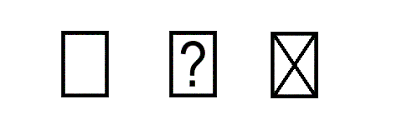
\includegraphics{Imagenes/BugsLQA/Notdef.png}
	\caption{Glifos con los que se representan habitualmente los caracteres no incluidos en una fuente}
	\label{Notdef}
\end{figure}
	
\subsection{Implementación de texto incorrecta}\label{ErrorImpIncorrecta}
Este error se produce cuando un texto que debería aparecer en un idioma se muestra en uno distinto, por ejemplo, alemán. Este error se puede producir porque hay texto equivocado documento de localización, o porque el programa tiene algún \textit{bug}. Debido a esto, el \textit{tester} tiene que verificar que la celda del documento tiene el texto adecuado.  
\subsection{Cadena no localizada}\label{ErrorNoLocalizada}
Este error se produce cuando un texto no está traducido. Puede deberse tanto a que el traductor no haya traducido el texto, como a que el desarrollador no haya facilitado dicho texto para la traducción. 
\subsection{Error tipográfico o de ortografía}\label{ErrorTypo}
Este error se produce cuando el texto tiene algún tipo de error ortográfico o errata.

\subsection{Error gramatical}\label{ErrorGramatical}
Este error se produce cuando el texto tiene un fallo gramatical.

\subsection{Error de traducción}\label{ErrorTraducción}
Este error se da cuando la traducción de un texto es errónea, ya sea por una traducción incorrecta (p. ej. ``Monedas de cobre'' a ``gold''); por falta de información u omisión de palabras; o porque el texto no tenga sentido en el contexto (p. ej al traducir desde el japonés).

\subsection{Solapamiento de texto}\label{ErrorSolapamiento}
Este error se produce cuando el texto sobresale de los límites de un botón o cuadro de diálogo. Puede deberse a una mala implementación por parte del desarrollador, o a que el traductor no ha respetado los límites de espacio que se le han dado.

\subsection{Truncamiento de texto}\label{ErrorTruncamiento}
Este error es el caso contrario al anterior. En este caso, el texto en lugar de salirse de los límites, queda cortado por ellos y no se muestra al completo.

\subsection{Error terminológico o incoherencia}\label{ErrorTermino}
Este error se produce cuando se usa una palabra incorrecta para referirse a una terminología clave (p. ej. utilizar el término ``grabar'' en lugar de ``guardar''). También puede darse cuando el mismo término no está escrito de la misma manera en dos lugares distintos (p. ej. Escribir un término importante en minúsculas en un lugar y en mayúsculas en otro.).

\subsection{Incumplimiento de directrices}\label{ErrorDirectrices}
Este error se da cuando una traducción no se cumplen las reglas de estilo que impone un distribuidor o plataforma para los videojuegos que se publiquen en ella. Por ejemplo, los mensajes del sistema en videojuegos en consolas deben de escribirse exactamente como aparecen en unas listas oficiales preparadas por las compañías que venden estas consolas.

\subsection{Error de subtítulos}\label{ErrorSubtitulos}
Este error tiene varias formas. Las más habituales son:
\begin{itemize}
	\item Los subtítulos no aparecen.
	\item Los subtítulos están desicronizados con el audio.
	\item No da tiempo a leer los subtítulos.
	\item Los subtítulos no están bien segmentados.
	\item Los subtítulos no coinciden con el contenido doblado. 
\end{itemize}

\subsection{Error de audio}\label{ErrorAudio}
Al igual que con los subtítulos, este error tiene varias formas:
\begin{itemize}
	\item El diálogo no se escucha o está en el idioma original
	\item El audio no está bien sincronizado con los gráficos.
	\item El audio no coincide con el contexto.
\end{itemize}

\subsection{Problemas culturales}\label{ErrorCultura}
Este error se suele dar cuando en un videojuego se utiliza alguna simbología o gesto que tiene un significado ofensivo en otra cultura. Un ejemplo puede ser la utilización del símbolo \textit{manji} en un juego japonés, que es muy parecido a la esvástica de la Alemania nazi.
\begin{figure}[h]
	
	\centering
	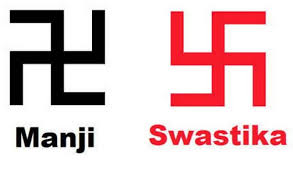
\includegraphics{Imagenes/BugsLQA/Manji.jpg}
	\caption{Comparación entre el \textit{manji} y la esvástica.}
	\label{Manji}
\end{figure}

%\begin{itemize}
%	\item Problema de fuente: La fuente utilizada no incluye alguno de los caracteres especiales de un idioma, por ejemplo las tildes (á), la ñ en español.
%	\item Implementación de texto incorrecta: Sucede cuando el texto debería aparecer en un idioma, aparece en un idioma diferente. Puede suceder por un descuido del desarrollador.
%	\item Cadena no localizada: Tiene lugar cuando la cadena de texto no viene traducida en el juego, puede deberse a un fallo del desarrollador.
	%\item Error tipográfico
	%\item Error gramatical
%	\item Error de traducción: Cuando el texto traducido no tiene el mismo significado que el texto original, o que no tiene sentido en ese contexto
	%\item Solapamiento de texto: Cuando el texto escrito es más largo de lo esperado por el programador por lo que se sale de los límites del espacio guardado para ese texto y se solapan. 
	%\item Texto truncado: Contrario al solapamiento de texto, el texto no se muestra de forma completa.
%	\item Error terminológico
%	\item Incoherencia
%	\item Incumplimiento de instrucciones: Tiene que ver con no seguir unas instrucciones del proyecto, por ejemplo en el mundo de las consolas, un tipo de error tiene que escribirse de una forma en concreta, saltarse esa norma supone retrasos en la aprobación del producto.
%	\item Error de estilo
%	\item Error subtítulos
%	\item Error de audio
%	\item Problemas culturales
%\end{itemize}

\section{Reconocimiento Óptico de Caracteres (OCR)}
El OCR (Reconocimiento Óptico de Caracteres, por sus siglas en inglés Optical Character Recognition) es una tecnología que convierte imágenes de texto manuscrito, impreso o mecanografiado en datos de texto que las computadoras pueden interpretar y manipular. En otras palabras, puede extraer el texto contenida en una imagen.

Para llegar al objetivo de reconocer el texto y extraerlo de la imagen el OCR da una serie de pasos	\footnote{(Extracting text from an image using Ocropus) \url{https://www.danvk.org/2015/01/09/extracting-text-from-an-image-using-ocropus.html} }	\footnote{(Improving the quality of the output) \url{https://tesseract-ocr.github.io/tessdoc/ImproveQuality.html} }:
\begin{enumerate}
	\item \textbf{Preprocesamiento de la imagen:}
	
	El propósito de este paso es procesar la imagen para que sea más legible para la computadora y reconocer así de forma mas eficiente los textos.
	\begin{itemize}
		\item Conversión a escala de grises: La mayoría de los OCR primero convierten la imagen en blanco y negro o escala de grises para simplificar el procesamiento.
		\item Reducción de ruido: Se aplican filtros para eliminar manchas, borrones o marcas en la imagen que puedan afectar la precisión del reconocimiento.
		\item Binarización: La imagen se convierte a una representación en blanco y negro, donde los píxeles se clasifican como parte del fondo (blanco) o del texto (negro). Este proceso ayuda a aislar los caracteres.
	\end{itemize}
	
	\item \textbf{Segmentación:}
	
	El OCR divide la imagen en secciones manejables. Primero separa líneas de texto.  Luego separa las palabras y finalmente descompone las palabras en caracteres individuales. Este paso es crucial, ya que el OCR necesita reconocer los caracteres de manera individual, pero considerando también su contexto dentro de una palabra o frase.
	
	\item \textbf{Detección de características:}
	
	Extracción de características de los caracteres: El OCR analiza los caracteres y sus formas, midiendo varios atributos como las líneas, contornos, cruces de líneas, y la disposición de los píxeles. Estos datos son usados para diferenciar letras, números y símbolos similares (como ``O'' y ``0'' o ``l'' y ``1'').
	Se aplican técnicas basadas en modelos geométricos, estructuras de redes neuronales o de aprendizaje automático para identificar patrones comunes en los caracteres.
	
	\item \textbf{Reconocimiento del carácter:}
	
	Clasificación de los caracteres: Una vez identificadas las características, el OCR las compara con una base de datos o ``alfabeto'' interno de posibles caracteres. Esto puede hacerse de varias maneras, dependiendo del tipo de OCR\footnote{(¿Qué es el reconocimiento óptico de caracteres (OCR)?) \url{https://aws.amazon.com/es/what-is/ocr/} }:
	\begin{itemize}
		\item Métodos basados en plantillas: Se compara cada carácter con un conjunto de plantillas predefinidas. Si la forma del carácter coincide con una plantilla, se clasifica como ese carácter.
		\item Métodos basados en aprendizaje automático o redes neuronales: Las técnicas modernas de OCR suelen usar redes neuronales entrenadas con miles de ejemplos de texto. El sistema ``aprende'' a identificar caracteres y a hacer distinciones más sutiles en base a sus experiencias pasadas.
	\end{itemize}

	
	
\end{enumerate}
